\documentclass[11pt]{article}
\usepackage{times}
\usepackage[letterpaper,margin=0.9in]{geometry}
\usepackage{booktabs}
\usepackage{longtable}
\usepackage{array}
\usepackage{tikz}
\usetikzlibrary{positioning,arrows.meta}
\pagestyle{plain}
\setlength{\parskip}{0.45em}
\setlength{\parindent}{0pt}
\raggedright
\renewcommand{\arraystretch}{1.25}

\title{A Speaker-Safe Pipeline for Detecting\\ Parkinson's Disease from Speech}
\author{Arannamoy Mondal}
\date{11 October 2026}

\begin{document}
\maketitle

\begin{abstract}
This note explains the full pipeline in plain English. The question is whether an elderly voice sounds like Parkinson's disease. Young controls stay on disk and are not labeled. The published score is computed on speakers, not on short windows. A flowchart shows the whole path. Tables then state what each of the one hundred steps does, and how you know that step is finished.
\end{abstract}

\section{The question}

Three groups sit in the corpus folder. Only two enter the experiment.

\begin{center}
\begin{tabular}{lrrl}
\toprule
Group & People & Files & Role \\
\midrule
Parkinson's disease & 28 folders, 25 people & 437 & Label 1 \\
Elderly healthy control & 22 & 349 & Label 0 \\
Young healthy control & 15 & 45 & Not used \\
\bottomrule
\end{tabular}
\end{center}

The young speakers are 19 to 29 years old and recorded only two readings plus a word list. The patients and the elderly controls are about 67 and recorded the same full protocol. Mixing the young group into the healthy class lets a model detect age and call it disease.

About 160 patient files from 2016 are stored at 44100 Hz. Every elderly file is stored at 16000 Hz. If that difference is left in the features, the model can detect the microphone. Every file is resampled to 16000 Hz before a feature is computed. A later run drops the 44100 Hz sessions and checks whether the score survives.

\begin{center}
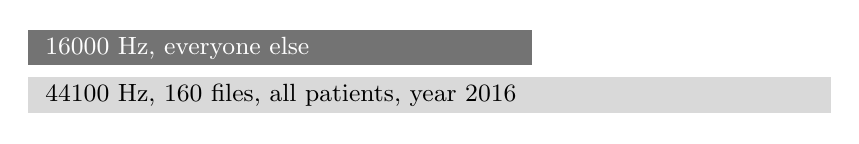
\begin{tikzpicture}
\fill[black!15] (0,0) rectangle (10.2,0.45);
\node[anchor=west,font=\small] at (0.1,0.22) {44100 Hz, 160 files, all patients, year 2016};
\fill[black!55] (0,0.6) rectangle (6.4,1.05);
\node[anchor=west,font=\small,text=white] at (0.1,0.82) {16000 Hz, everyone else};
\end{tikzpicture}
\end{center}

\section{The full pipeline}

Read this figure from top to bottom. A later box is not allowed to start until the box above it is true.

\begin{center}
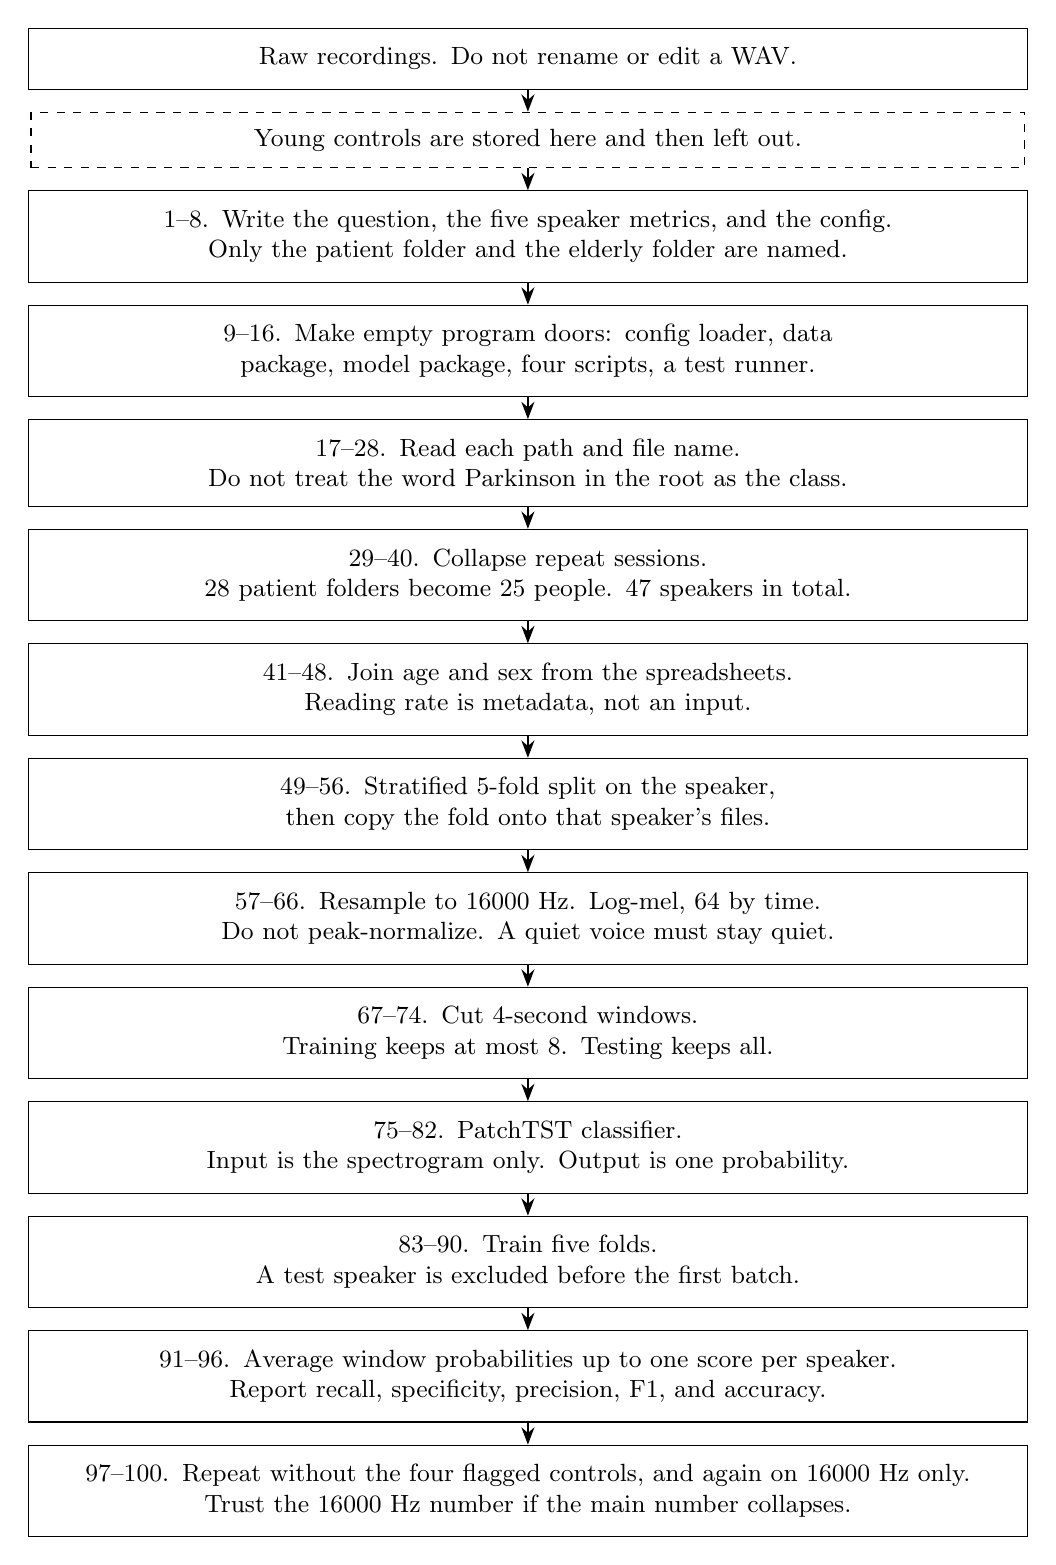
\begin{tikzpicture}[
  node distance=0.28cm,
  box/.style={draw, align=center, text width=12.2cm, inner sep=7pt, font=\small},
  side/.style={draw, dashed, align=center, text width=12.2cm, inner sep=6pt, font=\small},
  arr/.style={-{Stealth[length=2.2mm]}, thick}
]
\node[box] (raw) {Raw recordings. Do not rename or edit a WAV.};
\node[side, below=of raw] (young) {Young controls are stored here and then left out.};
\node[box, below=of young] (cfg) {1--8. Write the question, the five speaker metrics, and the config.\\ Only the patient folder and the elderly folder are named.};
\node[box, below=of cfg] (doors) {9--16. Make empty program doors: config loader, data package, model package, four scripts, a test runner.};
\node[box, below=of doors] (names) {17--28. Read each path and file name.\\ Do not treat the word Parkinson in the root as the class.};
\node[box, below=of names] (person) {29--40. Collapse repeat sessions.\\ 28 patient folders become 25 people. 47 speakers in total.};
\node[box, below=of person] (sheet) {41--48. Join age and sex from the spreadsheets.\\ Reading rate is metadata, not an input.};
\node[box, below=of sheet] (split) {49--56. Stratified 5-fold split on the speaker, then copy the fold onto that speaker's files.};
\node[box, below=of split] (audio) {57--66. Resample to 16000 Hz. Log-mel, 64 by time.\\ Do not peak-normalize. A quiet voice must stay quiet.};
\node[box, below=of audio] (win) {67--74. Cut 4-second windows.\\ Training keeps at most 8. Testing keeps all.};
\node[box, below=of win] (model) {75--82. PatchTST classifier.\\ Input is the spectrogram only. Output is one probability.};
\node[box, below=of model] (train) {83--90. Train five folds.\\ A test speaker is excluded before the first batch.};
\node[box, below=of train] (score) {91--96. Average window probabilities up to one score per speaker.\\ Report recall, specificity, precision, F1, and accuracy.};
\node[box, below=of score] (check) {97--100. Repeat without the four flagged controls, and again on 16000 Hz only.\\ Trust the 16000 Hz number if the main number collapses.};
\draw[arr] (raw) -- (young);
\draw[arr] (young) -- (cfg);
\draw[arr] (cfg) -- (doors);
\draw[arr] (doors) -- (names);
\draw[arr] (names) -- (person);
\draw[arr] (person) -- (sheet);
\draw[arr] (sheet) -- (split);
\draw[arr] (split) -- (audio);
\draw[arr] (audio) -- (win);
\draw[arr] (win) -- (model);
\draw[arr] (model) -- (train);
\draw[arr] (train) -- (score);
\draw[arr] (score) -- (check);
\end{tikzpicture}
\end{center}

\section{What one recording becomes}

A 2017 file name has four parts. The date is not part of the person code.

\begin{center}
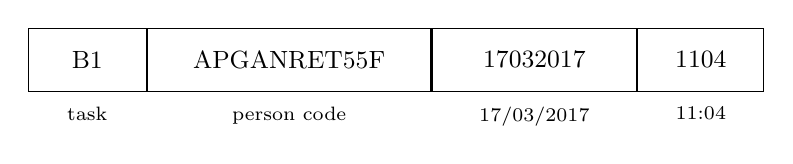
\begin{tikzpicture}[
  part/.style={draw, minimum height=8mm, align=center, font=\small, inner sep=3pt}
]
\node[part, minimum width=1.5cm] (t) at (0,0) {B1};
\node[part, minimum width=3.6cm, right=0pt of t] (k) {APGANRET55F};
\node[part, minimum width=2.6cm, right=0pt of k] (d) {17032017};
\node[part, minimum width=1.6cm, right=0pt of d] (c) {1104};
\node[font=\scriptsize, below=2pt of t] {task};
\node[font=\scriptsize, below=2pt of k] {person code};
\node[font=\scriptsize, below=2pt of d] {17/03/2017};
\node[font=\scriptsize, below=2pt of c] {11:04};
\end{tikzpicture}
\end{center}

A 2016 name is shorter at the end: six date digits, not eight. \texttt{260516} must be stored as 26/05/2016, not as the year 16.

After the name is read, the sound follows one path.

\begin{center}
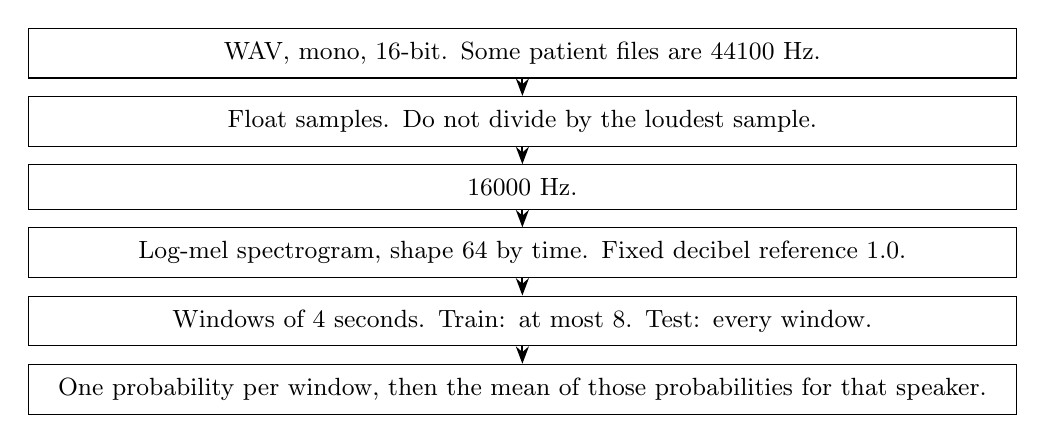
\begin{tikzpicture}[
  node distance=0.22cm,
  box/.style={draw, align=center, text width=12.2cm, inner sep=5pt, font=\small},
  arr/.style={-{Stealth[length=2.2mm]}, thick}
]
\node[box] (w) {WAV, mono, 16-bit. Some patient files are 44100 Hz.};
\node[box, below=of w] (r) {Float samples. Do not divide by the loudest sample.};
\node[box, below=of r] (s) {16000 Hz.};
\node[box, below=of s] (m) {Log-mel spectrogram, shape 64 by time. Fixed decibel reference 1.0.};
\node[box, below=of m] (n) {Windows of 4 seconds. Train: at most 8. Test: every window.};
\node[box, below=of n] (p) {One probability per window, then the mean of those probabilities for that speaker.};
\draw[arr] (w) -- (r);
\draw[arr] (r) -- (s);
\draw[arr] (s) -- (m);
\draw[arr] (m) -- (n);
\draw[arr] (n) -- (p);
\end{tikzpicture}
\end{center}

\section{The five numbers}

Each number answers a different question. They are computed only after the windows of one speaker have been averaged.

\begin{center}
\begin{tabular}{llp{7.2cm}}
\toprule
Name & Formula & What it answers \\
\midrule
Recall & TP / (TP + FN) & Of the patients, how many were caught? \\
Specificity & TN / (TN + FP) & Of the elderly controls, how many were left alone? \\
Precision & TP / (TP + FP) & Of the people called ill, how many were ill in this sample? \\
F1 & harmonic mean of precision and recall & Did we buy one of those by destroying the other? \\
Accuracy & (TP + TN) / all speakers & How often was the speaker call right? \\
\bottomrule
\end{tabular}
\end{center}

Recall and specificity are the clinical pair. F1 is the comparison number. Accuracy is reported, not trusted alone. Precision here is not the positive predictive value of a clinic, because this sample is about half patients and the community is not.

\section{Steps 1 to 8: freeze the decision}

\begin{longtable}{cp{6.4cm}p{6.4cm}}
\toprule
Step & What this step does & How you know it is done \\
\midrule
\endhead
1 & Write the question in one sentence: Parkinson's disease versus elderly healthy control, from speech. & The sentence does not mention the young group. \\
2 & Name the published score: speaker-level precision, recall, specificity, accuracy, and F1. & Window accuracy is listed only as a debug number. \\
3 & Record three citations: VoxTester 2016, IEEE Access 2017, DataPort DOI 10.21227/aw6b-tg17. & They are in the README, not only in a notebook. \\
4 & Point the config at the two group folders. & The young folder is absent from \texttt{groups}. \\
5 & Set rate 16000, tasks all, 5 folds, seed 42, group by speaker. & No other file contains these numbers. \\
6 & Ignore generated data, run outputs, the virtual environment, the corpus, and the zip. & A status listing does not show a WAV. \\
7 & Leave the WAV tree where it is. & No script writes inside it. \\
8 & Move the notebook to \texttt{notebooks/}. & The notebook is marked plots only. \\
\bottomrule
\end{longtable}

The phase is finished when the README states the cohort and the metric, and the config names exactly two groups.

\section{Steps 9 to 16: empty doors}

\begin{longtable}{cp{6.4cm}p{6.4cm}}
\toprule
Step & What this step does & How you know it is done \\
\midrule
\endhead
9 & \texttt{config.py} loads the yaml. & A missing key is reported. A missing value is not invented. \\
10 & Add the empty data package file. & \texttt{import patchtst.data} works. \\
11 & Add the empty model package file. & The file is empty. There is no network yet. \\
12 & Add the manifest script. & It loads the config and exits. It does not parse names. \\
13 & Add the feature-cache script. & It loads the config and exits. It does not read audio. \\
14 & Add \texttt{scripts/train.py}. & It loads the config and exits. It does not build a model. \\
15 & Add \texttt{scripts/evaluate.py}. & It loads the config and exits. It does not score anyone. \\
16 & Add a test runner and one test that fails on purpose. & The runner prints that failure. A missing test is not a pass. \\
\bottomrule
\end{longtable}

These four scripts look the same because their real jobs are not allowed yet. The file name reserves the door.

\section{Steps 17 to 28: read paths and names}

\begin{longtable}{cp{6.4cm}p{6.4cm}}
\toprule
Step & What this step does & How you know it is done \\
\midrule
\endhead
17 & Match \texttt{Elderly Healthy Control} and \texttt{People with Parkinson}. & The function does not search for the word Parkinson alone. \\
18 & Check an elderly path. & The label is 0. \\
19 & Check a patient path. & The label is 1. \\
20 & Check the dataset root. & It is refused. It is never labeled PD. \\
21 & Parse a 2017 name: eight date digits plus four time digits. & The date and the token are separate strings. \\
22 & Parse a 2016 name: six date digits plus four time digits. & The year is 2016, not 16. \\
23 & Map a leading \texttt{PR11} to \texttt{PR1}. & That file is not a new task. A normal PR1 file is unchanged. \\
24 & Remove a trailing double dot before \texttt{.wav}. & Alberto R's word-list file parses as 10/01/2017. \\
25 & Delete spaces inside the person code. & \texttt{VDIET AS47M} becomes \texttt{VDIETAS47M}. \\
26 & Read the task from the start of the name, longer codes first. & \texttt{FB1} is not read as \texttt{B1}. \\
27 & Walk only the two configured folders. & Young files never enter the table. \\
28 & Read rate, channels, format, and duration from the header. & The waveform is not loaded just to index the file. \\
\bottomrule
\end{longtable}

The phase is finished at 786 rows: 437 patient files and 349 elderly files. Every file is mono 16-bit PCM. About 160 patient files are 44100 Hz. Every elderly file is 16000 Hz.

\section{Steps 29 to 40: one person, one identity}

\begin{longtable}{cp{6.4cm}p{6.4cm}}
\toprule
Step & What this step does & How you know it is done \\
\midrule
\endhead
29 & Replace a stray person code with the code used by the rest of that folder. & Antonia G's \texttt{63F} file becomes \texttt{52F} and is flagged. \\
30 & Count that flag. & Exactly one file is flagged. \\
31 & Join folders with the same group and the same person code. & \texttt{VSIPTIOZ46M} is one person. \\
32 & Join folders with the same name and the same birth year and sex, even if the code spelling differs. & Nicola S and Roberto R each collapse. \\
33 & Do not join across groups. & An elderly code cannot merge with a patient code. \\
34 & Build the speaker id from the group plus the surviving code. & The id does not contain the folder path. \\
35 & Count speakers. & 47 speakers: 25 patients, 22 elderly. \\
36 & Check the three repeat people. & Each has two folders and both sample rates. \\
37 & Check the other Vito S. & The code ending \texttt{47M} is a different speaker id. \\
38 & Store native rate, duration, task, and session date on every row. & Later code does not parse the file name again. \\
39 & Write \texttt{data/manifest.csv} and \texttt{data/speakers.csv}. & A second run does not change the row count. \\
40 & Print the three linked speakers. & The merge is visible without opening the table. \\
\bottomrule
\end{longtable}

\section{Steps 41 to 48: join the spreadsheets}

\begin{longtable}{cp{6.4cm}p{6.4cm}}
\toprule
Step & What this step does & How you know it is done \\
\midrule
\endhead
41 & Read \texttt{TAB 5.xlsx} and \texttt{Tab 3.xlsx}, not the code legend. & Sex and age columns are found by name. \\
42 & Require sheet sex to equal the sex letter in the file name. & A mismatch stops the build. \\
43 & Match swapped elderly names: VITO L, LISCO G, SUMMO L. & All 22 elderly folders match. \\
44 & Match folder Mario B to the only Mario row. & He is not left unmatched. Age is within one year. \\
45 & Store sheet age and also session year minus birth year. & The two ages differ by at most 1 for every speaker. \\
46 & Flag Agnese P, Gilda C, Giovanna G, and Vitantonio D. & Only those four have \texttt{sheet\_flag}. \\
47 & Keep reading-rate columns as metadata. & No training function accepts them as input. \\
48 & Stop if any speaker has no sheet row. & A missing age is not filled with an empty value. \\
\bottomrule
\end{longtable}

The phase is finished when 47 of 47 speakers match and there are zero sex mismatches.

\section{Steps 49 to 56: split by speaker}

\begin{longtable}{cp{6.4cm}p{6.4cm}}
\toprule
Step & What this step does & How you know it is done \\
\midrule
\endhead
49 & Build folds from one row per speaker, not per file. & A person with 16 files is one unit. \\
50 & Use a stratified 5-fold split, shuffled, seed 42. & A plain group split on a patient-then-control sort is not used. \\
51 & Copy the fold onto every file of that speaker. & The column is the test fold. \\
52 & Check that no speaker appears in two folds. & A forgotten merge fails this check. \\
53 & Check that every fold contains both labels. & Each test fold has about 5 patients and 4 or 5 controls. \\
54 & Write \texttt{data/folds.csv}. & It has 47 rows. \\
55 & Add a switch to drop the four flagged controls. & The switch is off in the main run. \\
56 & Add a switch to keep only native 16000 Hz files. & This is the microphone run, not the main run. \\
\bottomrule
\end{longtable}

\section{Steps 57 to 66: make the spectrogram}

\begin{longtable}{cp{6.4cm}p{6.4cm}}
\toprule
Step & What this step does & How you know it is done \\
\midrule
\endhead
57 & Read samples as floating point on the file's own scale. & The audio is not divided by its loudest sample. \\
58 & Resample to 16000 Hz only when the stored rate differs. & A 16000 Hz file is not resampled twice. \\
59 & Check one 44100 Hz file. & Mel frames are about duration times 100, not times 441. \\
60 & Compute log-mel: 64 bands, Fourier size 512, window 400, hop 160. & The shape is 64 by time. \\
61 & Use a fixed decibel reference of 1.0. & A quiet file stays quieter than a loud file. \\
62 & Name each cache file by a hash of the WAV path. & Changing the task list cannot attach the wrong array. \\
63 & Reuse a cache file only if its first dimension is 64. & A changed band count recomputes it. \\
64 & Write the cache path back into the manifest. & 786 paths exist. \\
65 & Keep feature settings in the config, not in the audio code. & Changing the hop means editing the yaml only. \\
66 & Time one full cache and write the seconds down. & You know whether training must read the cache. \\
\bottomrule
\end{longtable}

A 73-second file that began at 44100 Hz has about 7300 frames. A 6-second syllable file has about 600.

\section{Steps 67 to 74: cut windows}

\begin{longtable}{cp{6.4cm}p{6.4cm}}
\toprule
Step & What this step does & How you know it is done \\
\midrule
\endhead
67 & Define one window as 4.0 seconds, 400 frames, hop 2.0 seconds. & Both numbers come from the config. \\
68 & Pad a short clip by repeating the edge. & The shortest vowel still yields one window. \\
69 & In training, keep at most 8 windows, evenly spaced. & A 250-second reading does not yield 100 windows. \\
70 & In testing, keep every window. & The cap is not applied in evaluation. \\
71 & Copy the file label and the speaker id onto each window. & The dataset never receives a folder name. \\
72 & Check the batch shape. & It is count, then 64, then 400. \\
73 & Refuse a batch that mixes two folds. & The dataset is built from one split. \\
74 & Let the config choose all tasks or a shorter list. & Vowels only does not rebuild speaker ids. \\
\bottomrule
\end{longtable}

Do not start the network before this check: one long patient file contributes 8 training windows and more than 8 test windows.

\section{Steps 75 to 82: the classifier}

\begin{longtable}{cp{6.4cm}p{6.4cm}}
\toprule
Step & What this step does & How you know it is done \\
\midrule
\endhead
75 & Add the training library. & The data package still imports without it. \\
76 & Cut time into patches. Length and stride come from the config. & The 64 channels stay independent. \\
77 & Put a classification head on the encoder. & The output is one logit, not a forecast. \\
78 & Write the input contract in words. & A batch of 64 by 400 goes in. One probability comes out. \\
79 & Run one dummy batch on the CPU. & The output shape is batch size by 1. \\
80 & Save the patch length beside the checkpoint. & It is not guessed later from the weight file. \\
81 & Accept only the spectrogram. & Sex, age, reading rate, and native rate are not inputs. \\
82 & Count the parameters and write the number down. & The model is not larger than 47 speakers can support. \\
\bottomrule
\end{longtable}

\section{Steps 83 to 90: train}

\begin{longtable}{cp{6.4cm}p{6.4cm}}
\toprule
Step & What this step does & How you know it is done \\
\midrule
\endhead
83 & Train one fold. & Test speakers are excluded before the first batch. \\
84 & Write the run to its own dated folder, with the fold and a config hash. & A second run does not overwrite the first. \\
85 & Copy the yaml into that folder. & The copy is the config that was used, not a later edit. \\
86 & Save the checkpoint there. & The path is in a small run file. \\
87 & Write the loss for each epoch in that folder. & The notebook is not the log. \\
88 & Balance the loss. & 437 patient files do not silently outweigh 349 elderly files. \\
89 & Stop early on a validation speaker loss. & Early stopping cannot see the test fold. \\
90 & Repeat for folds 0 through 4 with the same seed. & Five run folders exist. \\
\bottomrule
\end{longtable}

Opening any run folder must show the fold, the seed, and the config hash without reading the source code.

\section{Steps 91 to 100: the score, and whether it is real}

\begin{longtable}{cp{6.4cm}p{6.4cm}}
\toprule
Step & What this step does & How you know it is done \\
\midrule
\endhead
91 & Score every test window. & The window table has speaker id, path, task, and probability. \\
92 & Average probabilities by file, then by speaker. & The speaker score table exists. \\
93 & Compute the five metrics on speaker scores. & The metrics file exists. The threshold was not chosen on the test fold. \\
94 & Pool the five test folds and compute the five numbers once. & This pooled number is the one you quote. \\
95 & Also report the mean and the spread across folds. & The best fold is not quoted. \\
96 & Compare the speaker count in the score table with the test speakers. & A dropped speaker fails the run. \\
97 & Repeat evaluation without the four flagged controls. & You record whether the pooled F1 moves. \\
98 & Retrain and evaluate on native 16000 Hz only. & The seven patients who exist only at 44100 Hz are gone. \\
99 & If that F1 collapses, write it in the run note. & The mixed-rate number is not published as the disease result. \\
100 & Plot from the speaker score table only. & The notebook does not open a WAV except through that table. \\
\bottomrule
\end{longtable}

Three numbers then sit side by side: the main pooled F1, the F1 without the four flagged controls, and the F1 on 16000 Hz only. The third is the number that is trusted if the first was helped by the old microphone.

\begin{thebibliography}{9}
\bibitem{vox} G.~Dimauro, D.~Caivano, V.~Bevilacqua, F.~Girardi, and V.~Napoletano, ``VoxTester, software for digital evaluation of speech changes in Parkinson disease,'' IEEE MeMeA, 2016.
\bibitem{access} G.~Dimauro, V.~Di Nicola, V.~Bevilacqua, D.~Caivano, and F.~Girardi, ``Assessment of Speech Intelligibility in Parkinson's Disease Using a Speech-To-Text System,'' IEEE Access, 2017.
\bibitem{dataport} G.~Dimauro and F.~Girardi, ``Italian Parkinson's Voice and Speech,'' IEEE DataPort, 2019. DOI 10.21227/aw6b-tg17.
\end{thebibliography}

\end{document}
